\documentclass[12pt, twocolumn]{article}
\usepackage{graphicx}
\usepackage{lipsum}
\usepackage{hyperref}
\usepackage{xcolor}
\usepackage{amsmath, amssymb}
\usepackage{cuted}
\usepackage{amsbsy}
\usepackage[margin=0.7in]{geometry}
\usepackage[style=numeric-comp,useprefix,hyperref,backend=bibtex]{biblatex}
\graphicspath{{../img/}}
\usepackage{endnotes}
\usepackage{float}
\title{Wine Project Report}
\author{Ruggero Nocera (SXXXXX1) \\ Quarta Matteo (SXXXXXX)}
\date{}


\begin{document}

\maketitle
\begin{strip}
    {\bf Abstract}
    This paper is an analysis of the effectiveness of the various models studied during the course applied to a binary classification model.
    The dataset is a transformed version of the one provided in {\it Modeling wine preferences by data mining from physicochemical properties}
    from {\it Decision Support Systems, Elsevier} (P. Cortez, A. Cerdeira, F. Almeida, T. Matos and J. Reis.), where grades span from 0 to 10. 
    Grade 6 has been removed, grades above 6 have been mapped to class 1 and grades below 6 to class 0.
    Due to limited time and computanional power, results may be just close-to or far-from optimal, depending on the time required to train a model.
\end{strip}
\tableofcontents


\section{Preliminary Data Analysis}
\subsection{Feature Distribution}

Before discussing the model, their implementation and their effectiveness we briefly take a look at how the features are distributed.
For convenience we shall now report the legend just one, but keep in mind that in all pictures red color is associated to class 0 (which we will be referring to as class {\it Bad}) and green color is associated to class 1 (which will be class {\it Good}).

\begin{figure}[H] 
    \caption{Histogram of Class' Features}
    \label{fig:disthist}
    {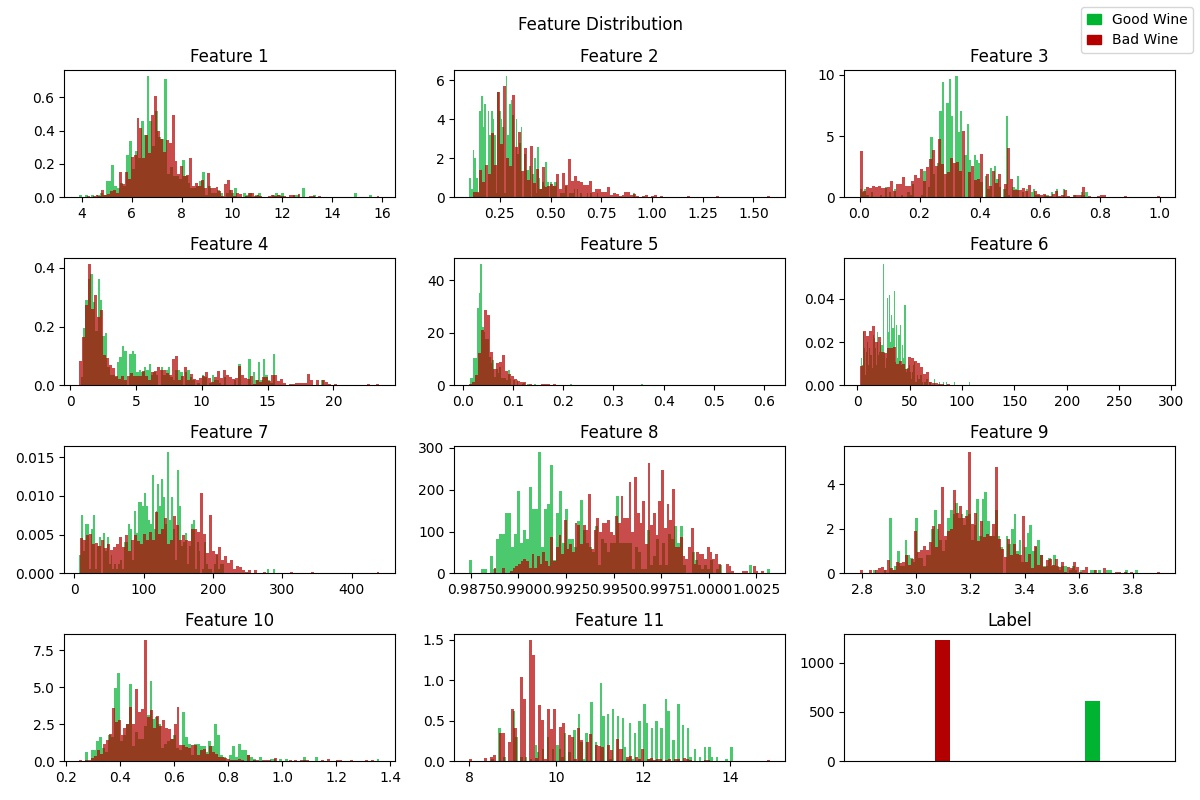
\includegraphics[width=\linewidth]{dist.jpg}}
\end{figure}

First of all, our training dataset is unbalanced. 
In the next pages we will be classifying samples obtained from a K-Fold\footnotemark Validation approach, using a theoretical threshold given by:

$$ t = -\log{\frac{\pi}{1-\pi}} $$

For the threshold to be optimal, we should use the empirical prior $\pi \approx .33$ based on a frequentist approach;
Instead we will be using a non-optimal prior $\tilde{\pi} = .5$ as it is the application we are going to be targeting
.
\footnotetext{K varies through models. For fast ones, 5 or 10 is used. For slower ones, 3 is used.}

Coming back to features distributions, some things are to be noticed.
While some features are similar between class Good and class Bad (see feature {\it 1}) others differ substantially and can be very helpful in discriminating samples (see feature {\it 8}).

Moreover, the features are distributed in various ways: while some do look pretty Gaussian (see feature {\it 9}) and others are instead fairly regular (see feature {\it 5}) and could thus be well estimated by Gaussian models\footnotemark , other act in a more irregular way.

\footnotetext{Meaning both Gaussian Classifiers and Gaussian Mixture Models}.

To take a closer look we now project the data on the two dimensional plane. 
We will be using 3 methods to do so: PCA\footnotemark , Normalization + PCA, Normalization + Whitening.

\footnotetext{Without data centering to appreciate the correlation}

\begin{figure}[H]     
    {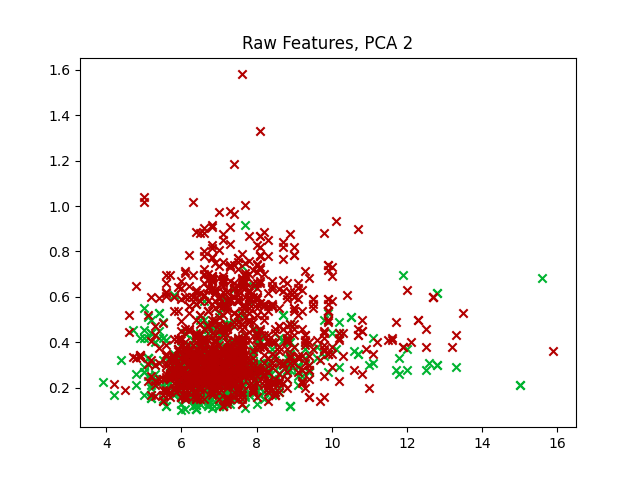
\includegraphics[width=\linewidth]{2DRAW.png}}
    \caption{2D-PCA Projection}
    \label{fig:2DRAW}
\end{figure}

The points are very close one another, we thus expect linear models to be not so effective compared to others.
The data is pretty {\it circularly} distributed, so correlation may not play an important role in discriminating samples.

\begin{figure}[H] 
    {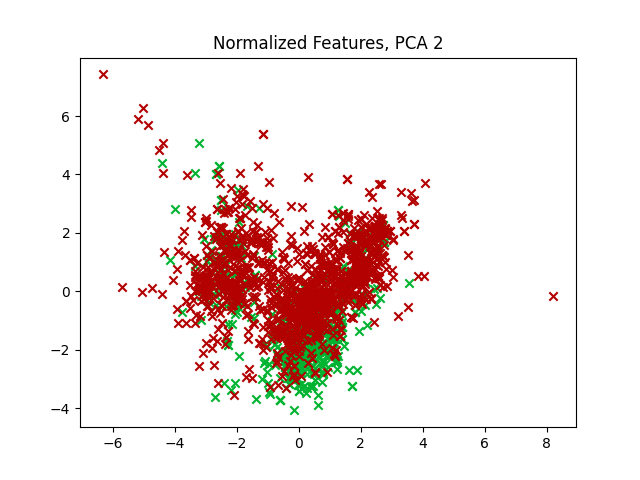
\includegraphics[width=\linewidth]{2DNorm.png}}
    \caption{2D-PCA Projection, Normalized Data}
    \label{fig:2DNORM}
\end{figure}

The normalized projection seems to split data in two clusters, each containing some samples of either class, but some points of different class seem to get far apart from the other.
So normalization is a technique worth trying.

Note that for Normalization we refer to {\it Z-Normalization}. 
From some early tests we found that {\it Min-Max} normalization was not very effective, and with {\it Gaussianization} centering and scaling data in the same way as Z while being slower, we decided to use this method.

Lastly we take a look at normalized and whitened data.

\begin{figure}[H] 
    {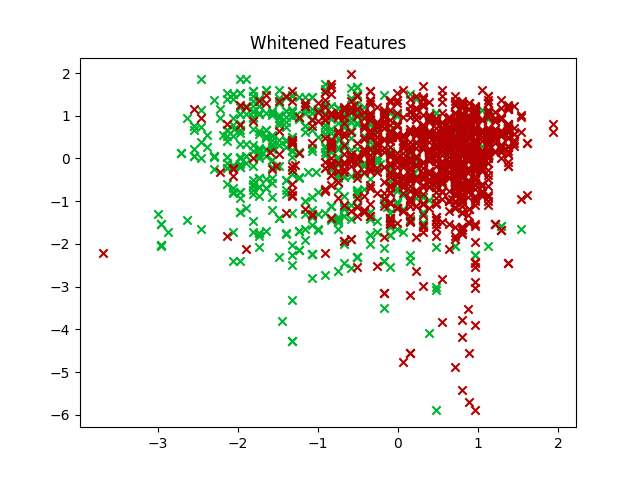
\includegraphics[width=\linewidth]{2DWhitened.png}}
    \label{fig:2DWHI}
    \caption{2D-PCA Projection, Whitened Data}
\end{figure}

Results do look interesting: points to get much apart, even if we can spot many outliers.
With the distribution being this way, we could expect even linear models to achieve decent results.


\section{Pre-Processing Analysis}

In this section we will run some dummy\footnotemark models to learn how pre-processing affects the models for our task.
\footnotetext{Simple model that run with arbitrary, non-optimized hyper-parameters}

Note that we will be discarding combinations or entire models targeting our final application.
A discussion about different applications will be made in the ending.

\subsection{Pre-Processing MVG Classifiers}

Since MVG classifiers are fairly similar, 
we will now pick the most promising one and discarding the others, 
while trying to infer its optimal working condition.

\begin{table}[H] 
    \centering
    \begin{tabular}{||c|c|c|c||}
        \hline
        Type & PCA & DCF & minDCF \\
        \hline
        \hline
        Raw   & 8  & 0.375 & {\bf 0.321} \\
        Raw   & 9  & {\bf 0.360} & 0.326 \\
        Norm. & 10 & 0.419 & 0.330 \\
        Norm. & 11 & 0.424 & 0.322 \\
        Whit. & 11 & 0.424 & 0.322 \\
        Whit. & 8  & 0.392 & 0.342 \\
        \hline
    \end{tabular}
    \caption{Full-Covariance MVG - Best Results}
    \label{fullcovtab}
\end{table}

    
\begin{table}[H] 
    \centering
    \begin{tabular}{||c|c|c|c||}
        \hline
        Type & PCA & DCF & minDCF \\
        \hline
        \hline
        Raw   & 11 & {\bf 0.342} & 0.332 \\
        Norm. & {\bf 5}  & 0.414 & {\bf 0.330} \\
        Norm. & 11 & {\bf 0.342} & 0.332 \\
        Whit. & 11 & {\bf 0.342} & 0.332 \\
        \hline
    \end{tabular}
    \caption{Tied-Covariance MVG - Best Results}
    \label{tiedcovtab}
\end{table}

\begin{table}[H]
    \centering
        \begin{tabular}{||c|c|c|c||}
            \hline
            Type & PCA & DCF & minDCF \\
            \hline
            \hline
            Raw   & 9  & 0.404 &  0.365 \\
            Raw   & 7  & {\bf 0.391} &  0.370 \\
            Norm. & 9  & 0.428 &  0.350 \\
            Whit. & 11 & 0.460 &  {\bf 0.344} \\
            Whit. & 5  & 0.394 &  0.374 \\
            \hline
    \end{tabular}
    \caption{Naive-Bayes MVG - Best Results}
    \label{naivetab}
\end{table}

The results seem in line with our assumptions.
In fact, if  we look again at picture \ref{fig:2DRAW} we wouldn't expect the Naive Bayes to perform much differently from the Full Covariance one.
The best model, with a modest margin, is the tied covariance one so we will keep it,
and removing some dimensions seems to be helpful.

Notice that while the Tied Covaraiance model achieved the best DCF\footnotemark of all classifiers,
the MVG achieved the lowest Minimum DCF values, hiting that it is actually the one out of the three that could theoretically best separate classes.
\footnotetext{By DCF we actually mean the {\it normalized} DCF, considering a prior $\pi_T = .5$ and equal costs}

Normalization and Whitening look irrelevant so we won't further experiment them.

\subsection{Pre-Processing for GMMs}

For our dummy GMM model we arbitrairly set the number of components to 4.
The starting point for our EM algorithm is identity covariance matrices and means placed around the dataset mean.

\begin{table}[H]
    \centering
        \begin{tabular}{||c|c|c|c||}
            \hline
            Type & PCA & DCF & minDCF \\
            \hline
            \hline
            Raw & No & 0.410 & {\bf 0.394}  \\
            Normalized &  9 & {\bf 0.407} & 0.402 \\
            Whitened & 4 & 0.429 & 0.420 \\
            \hline
    \end{tabular}
    \caption{GMM - Best Results}
    \label{tab:gmmresults}
\end{table}

As for our Gaussian Classifiers, Whitening and Normalization do not look promising. 
However, as the difference between the Raw and Normalized does not look significant,
we will further test both models.
This first test shows us that high dimensionality is actually preferred.

\subsection{Pre-Processing for Polynomial Kernel SVMs}

The polynomial kernel function is defined as:

$$ \phi({\bf x}_1)^T\phi({\bf x}_2) = k({\bf x_1}, {\bf x_2}) = ({\bf x}_1^T{\bf x}_2 + c)^d + b $$

We proceed to set our parameters arbitrairly for this dummy execution:

$$k({\bf x_1}, {\bf x_2}) = ({\bf x}_1^T{\bf x}_2+1)^2+0.5 $$

\begin{table}[H]
    \centering
        \begin{tabular}{||c|c|c|c||}
            \hline
            Type & PCA & DCF & minDCF \\
            \hline
            \hline
            Raw & 7 & 0.554 &  0.545  \\
            Normalized & 6 & {\bf 0.393} &  {\bf 0.381}  \\
            Whitened & 11 & 0.399 &  0.393  \\
            \hline
    \end{tabular}
    \caption{Polynomail Kernel SVM - Best Results}
\end{table}

While competitiveness with other models has to be made later, when each one will be fully used, here we see an interesting change:
normalization greatly improves our classification.
While a lower PCA has obtained the lowest DCF, it is not significantly lower than the one obtained with higher dimensionality, so we can say that here it's normalization helping us out.
Whitening, again, does not make any difference, as the results are same or close to the ones obtained with normalization only.

Notice also how scores seems well calibration with our theoretical threshold even if they do not have a probabilistic interpretation.

\subsection{Pre-Processing for RBF Kernel SVMs}

The dummy RBF function used here is the following:

$$\displaystyle k({\bf x_1}, {\bf x_2}) = e^{-\gamma||{\bf x}_1 - {\bf x}_2||^2} + b = e^{-0.05||{\bf x}_1 - {\bf x}_2||^2} + 0.05 $$

Small values of $\gamma$ and $b$ were picked to avoid numerical issues when using non-normalized models.

\begin{table}[H]
    \centering
        \begin{tabular}{||c|c|c|c||}
            \hline
            Type & PCA & DCF & minDCF \\
            \hline
            \hline
                Raw & 10 & 0.588 & 0.579 \\ 
                Normalized & 11 & {\bf 0.356} & {\bf 0.352} \\ 
                Whitened & 11 & {\bf 0.356} & {\bf 0.352} \\ 
            \hline
    \end{tabular}
    \caption{RBF Kernel SVM - Best Results}
\end{table}

Just like polynomial kernel, RBF prefers high dimensionality , so further testing in this direction is required.
Again, normalization plays an important role while whitening seems to have no effect whatsoever and scores look extremely well calibrated.

Just like polynomial kernel SVMs, here normalization has no effect whatsoever whilte normalization greatly improves our performance.
The RBF Kernel works significantly better when working with all or most components. 

We are not yet discussing perfomance in detail but so far, this is our most promising model.

\subsection{Pre-Processing for Logistic Regression Model}

Regarding the Logistic Regression, we will consider both linear and quadratic model.

\subsubsection{Linear Logistic Regression}

In the Linear model, dimensionality reduction through PCA and prepocessing through normalization
helped to obtain lower minimum DCF compared to raw features.
For the whitened features, best results are obtained without applying PCA.
As the Gaussian Classifiers, only a small numberof features can be removed.

Only results with already optimized hyperparameters are reported.
\begin{table}[H]
    \centering
    \tiny
        \begin{tabular}{||c|c|c|c||}
            \hline
            Type & PCA & DCF & minDCF \\
            \hline
            \hline
            Raw ($\lambda = 0.0001$) & 10 & 0.369 &  0.342  \\
            Normalized ($\lambda = 0.01$) & 9 & 0.369 &  {\bf 0.336}  \\
            Whitened ($\lambda = 0.0001$) & 11 & 0.549 &  0.503  \\
            \hline
    \end{tabular}
    \caption{Linear Logistic Regression - Best Results}
\end{table}

Whitening didn't help so much to improve results, so it won't be considered in further analysis.
\subsubsection{Quadratic Logistic Regression}

In the Quadratic Logistic Regression, after the preprocessing stage, the features space
was expanded through 
$$ {\bf \boldsymbol{\phi}(x)} = {
    \begin{bmatrix}
    vec\langle{\bf xx^T}\rangle\\
    {\bf x}
    \end{bmatrix}}
$$ 

In contrast to linear model, whitening helped as well as normalization, PCA
was useful in both cases, with and without preprocessing, but with a notable difference
in the number of features used to obtain following results.

\begin{table}[H]
    \tiny
    \centering
        \begin{tabular}{||c|c|c|c||}
            \hline
            Type & PCA & DCF & minDCF \\
            \hline
            \hline
            Raw ($\lambda = 0.1$) & 6 & 0.385 &  0.366  \\
            Normalized ($\lambda = 0.001$) & 10 & 0.324 &  {\bf 0.307}  \\
            Whitened ($\lambda = 0.001$) & 10 & 0.324 &  {\bf 0.307}  \\
            \hline
    \end{tabular}
    \caption{Quadratic Logistic Regression - Best Results}
\end{table}

\subsection{Pre-Processing for Linear SVM}

The Linear SVM model performed much better with normalization and whitening rather than raw features.
Applying PCA was useful to obtain low values of minimum DCF in all cases, even if the model trained
with raw features performed worse than models trained with preprocessed features.

\begin{table}[H]
    \centering
    \tiny
        \begin{tabular}{||c|c|c|c|c|c||}
            \hline
            Type & K & C & PCA & DCF & minDCF \\
            \hline
            \hline
            Raw & 0 & 10.0 & 6 & 0.911 &  0.568  \\
            Normalized & 10 & 0.1 & 9 & 0.350 &  {\bf 0.330}  \\
            Whitened & 1.0 & 1.0 & 9 & 0.364 &  0.331  \\
            \hline
    \end{tabular}
    \caption{Linear SVM - Best Results}
\end{table}

The high difference between minimum DCF and DCF suggests us that scores are miscalibrated, but we will try to
optimize it in next chapters.

\section{Optimizing Models}

\subsection{Optimizing Logistic Regression}

Now we will try to find the $\lambda$ that gives us the best (lower) minimum DCF in the validation set, extracted
from the training set through a 5-fold cross validation protocol.
Several values of $\lambda$ have been tried, in a range between $\left[10^{-4}, 10^3\right]$ for both linear and quadratic model.

\begin{table}[H]
    \tiny
    \centering
        \begin{tabular}{||c|c|c|c|c|c||}
            \hline
            Model & Type & $\lambda$ & PCA & DCF & minDCF \\
            \hline
            \hline
            Linear & Normalized & 0.01 & 9 & 0.369 &  0.336  \\
            Quadratic & Normalized & 0.001 & 10 & 0.324 &  0.307  \\
            \hline
    \end{tabular}
    \caption{Best $\lambda$ values for Logistic Regression}
\end{table}

We tried to lower the difference between the DCF and the minimum one, in both linear and and quadratic model.
To reduce the DCF, we tried to calibrate the scores:

\begin{table}[H]
    \tiny
    \centering
        \begin{tabular}{||c|c|c|c|c|c||}
            \hline
            Model & Type & $\lambda$ & PCA & DCF & minDCF \\
            \hline
            \hline
            Linear & Normalized & 0.01 & 9 & \textcolor{red}{0.373} &  0.336  \\
            Quadratic & Normalized & 0.001 & 10 & \textcolor{green}{0.312} &  0.307  \\
            \hline
    \end{tabular}
    \caption{Calibrated scores for logistic regression}
    \label{logregcalibration}
\end{table}

As reported in table \ref{logregcalibration}, calibration helped in the quadratic case, 
but DCF got worse in linear one.

\subsection{Optimizing MVG Classifiers}

Since the MVG Classifiers we will be only briefly discussing score calibration.
In particular we will focus on Full-Covariance and Naive Bayes MVG Classifiers, as Tied Covariance already is very close to being optimal.

The scores will be rebalanced using logistic regression as it follows:


\begin{equation}
    f(s) = \alpha s + \beta
\end{equation}

The scores are the ones that produced the best result for both models as in table \ref{fullcovtab} and \ref{naivetab}. 

\begin{table}[H]
    \centering
        \begin{tabular}{||c|c|c||}
            \hline
            minDCF & $DCF_{Before}$ & $DCF_{After}$ \\
            \hline
            \hline
            0.362 & 0.401 & \textcolor{green}{\bf0.390} \\ 
            0.367 & {\bf 0.383} & \textcolor{red}{\bf 0.412} \\ 
            \hline
    \end{tabular}
    \caption{MVG Recalibrated Scores DCFs}
    \label{mvgcalibration}
\end{table}

Recalibration heavily damages our Naive Bayes classifiers so it's not a good choice.
The Full Covariance one has a modest DCF decrement, but it's still worse than the plain Naive Bayes one.
Lastly, by looking at table \ref{tiedcovtab}, we notice that both models perform worse than our Tied Covariance one, so we will be discarding them in our final evaluation.

\subsection{Optimizing Gaussian Mixture Models}

For GMMs we decided from table \ref{tab:gmmresults} to inspect both raw and normalized optimization.

\begin{table}[H] 
    \centering
    \begin{tabular}{||c|c|c|c|c||}
        \hline
        Type & DCF & DCF$_{min}$ & PCA & \# Comp. \\
        \hline
        \hline
        Raw  & {\bf 0.347} & {\bf 0.308} & No & 2 \\
        Norm & 0.365 & 0.311 & 6  & 3 \\
        Norm & 0.348 & 0.317 & No & 2 \\
        \hline
    \end{tabular}
    \caption{GMM Optimization Results}
    \label{tab:gmmoptimization}
\end{table}



\begin{table}[H] 
    \centering
    \begin{tabular}{||c|c|c|c||}
        \hline
        Type & minDCF & DCF$_{Before}$ & DCF$_{After}$ \\
        \hline
        \hline
        Norm. & 0.316 & 0.346 & \textcolor{green}{\bf 0.324} \\
        Raw & 0.328 & 0.348 & \textcolor{green}{\bf 0.334} \\
        \hline
    \end{tabular}
    \caption{GMM Optimization Results}
    \label{tab:gmmcalibration}
\end{table}

Contrary to what we have seen in table \ref{tab:gmmresults}, here the scores are fairly distant from the minimum possible DCF, and recalibrating the scores did indeed help.

The normalized GMM is the best one, but data does not suggest that in general normalized GMMs are better, so both model will be used later on.

\section{Experimental Results}

After having run our models in order to find the best parameters, we now test them on previously unseen data.

All the parameters here reported have been found through a K-Fold Cross-Validation approach.
The value of K used spans from 3 (heavier models, e.g. Kernel SVMs) up to 10 (lighter models, e.g. Gaussian Classifiers).

\begin{table*}[t] 
    \centering
    \begin{tabular}{||c|c|c|c|c|c||}
        \hline 
        Model & Features & PCA & Hyper-Parameters & DCF & DCF$_{min}$ \\
        \hline
        - & - & - & - &  - & - \\
        \hline
    \end{tabular}
\end{table*}

\newpage

As mentioned earlier, up to now all models have been evaluated considering a balanced application ( $pi_T = 0.5$ ).
We now want to discuss how or best models, based on the table above, perform in different conditions.

....


\end{document}